\chapter{Leptoquark Search at the LHC}
\label{chapter:LQ_search}

\section{Leptoquark Models and Phenomenology}
\label{sec:leptoquarks}

\subsection{General properties of leptoquarks}
\label{subsec:lq_general}

Leptoquarks~(LQs) are hypothetical colour-charged bosons that couple directly to a quark and a lepton and therefore mediate interactions connecting the quark and lepton sectors.
Depending on their spin, leptoquarks can be classified as scalar leptoquarks with spin zero or vector leptoquarks with spin one. 
They appear in several theoretical frameworks, including grand unified theories such as $SU(5)$ and $SO(10)$, quark--lepton unification models such as the Pati--Salam model, composite models, and models motivated by flavour anomalies~\cite{GeorgiGlashow1974SU5,PatiSalam1974,Dorsner2016}.


Leptoquarks are particularly interesting in the context of semileptonic flavour physics. 
Their tree-level exchange can generate effective four-fermion interactions involving two quark fields and two lepton fields. 
Such interactions can modify flavour observables in processes such as $b\rightarrow c\tau\nu$ and $b\rightarrow s\ell^{+}\ell^{-}$. 
In addition, the flavour structure of LQ couplings is model dependent and can be arranged to favour interactions with third-generation fermions. 
This feature is motivated by the distinctive role of the top quark, bottom quark, and $\tau$-lepton in many flavour-motivated scenarios.

At the LHC, leptoquarks can be searched for directly. 
Since they carry colour charge, they can be pair-produced through QCD interactions. 
Additional production modes, such as single production or non-resonant exchange, are also possible, depending on the LQ coupling to SM quarks and leptons. 
Therefore, the LQ searches in ATLAS provide information complementary to low-energy flavour measurements: flavour observables probe virtual effects through precision measurements, while the search at $pp$ collider probes direct LQ production or high-energy virtual exchange.

% \subsection{Nomenclature and Classification}
% \label{subsec:lq_classification}

% A standard classification of scalar and vector leptoquark representations was introduced by Buchmuller, Rueckl and Wyler~\cite{BRW1987}. 
% In this thesis, the representations are denoted using the notation commonly adopted in recent leptoquark reviews~\cite{Dorsner2016}. 
% Each leptoquark representation is labelled by its transformation properties under the SM gauge group,
% $SU(3)\times SU(2)\times U(1)$.
% For example, a representation written as
% $(3,2,1/6)$
% denotes a field that transforms as a triplet under the colour group $SU(3)$, as a doublet under the weak-isospin group $SU(2)$, and has weak hypercharge $Y=1/6$. 
% The two components of the $SU(2)$ doublet have $T^{3}=+1/2$ and $T^{3}=-1/2$, respectively. 
% Using the relation $Q=T^{3}+Y$, their electric charges are therefore
% \begin{align}
%     Q=+\frac{1}{2}+\frac{1}{6}=\frac{2}{3},
%     \qquad
%     Q=-\frac{1}{2}+\frac{1}{6}=-\frac{1}{3}.
% \end{align}
% Thus, the representation $(3,2,1/6)$ describes a colour-triplet weak doublet with two electric-charge components.
% Beyond that, an additional marking is introduced: A tilde on the LQ name, such as $\tilde{R}_{2}$ or $\tilde{S}_{1}$, denotes a distinct LQ representation with a different hypercharge.
% The scalar and vector LQ representations are shown in Table~\ref{tab:lq_reps}. 

% \begin{table}[htbp]
%     \centering
%     \caption[List of scalar and vector LQs]{List of scalar and vector LQs and their gauge representation~\cite{Dorsner2016}.}
%     \label{tab:lq_reps}
%     \begin{tabular}{ccc}
%         \toprule
%         Spin & Symbol & $(SU(3), SU(2), U(1))$ \\
%         \midrule
%         0 & $S_{1}$ & $(\bar{3},1,1/3)$ \\
%         0 & $\tilde{S}_{1}$ & $(\bar{3},1,4/3)$ \\
%         0 & $S_{3}$ & $(\bar{3},3,1/3)$ \\
%         0 & $R_{2}$ & $(3,2,7/6)$ \\
%         0 & $\tilde{R}_{2}$ & $(3,2,1/6)$ \\
%         \midrule
%         1 & $U_{1}$ & $(3,1,2/3)$ \\
%         1 & $\tilde{U}_{1}$ & $(3,1,5/3)$ \\
%         1 & $U_{3}$ & $(3,3,2/3)$ \\
%         1 & $V_{2}$ & $(\bar{3},2,5/6)$ \\
%         1 & $\tilde{V}_{2}$ & $(\bar{3},2,-1/6)$ \\
%         \bottomrule
%     \end{tabular}
% \end{table}

% The gauge representation of a leptoquark determines which gauge-invariant quark--lepton interactions can be written. 
% For example, the vector singlet $U_{1}\sim(3,1,2/3)$ can couple to the left-handed bilinear $\bar{Q}_{L}\gamma^{\mu}L_{L}$. 
% After expanding the weak doublets, this interaction contains both $\bar{u}_{L}\gamma^{\mu}\nu_{L}$ and $\bar{d}_{L}\gamma^{\mu}e_{L}$ terms, leading to decay modes involving either charged leptons or neutrinos. 
% In contrast, an $SU(2)$-triplet LQ contains three components with different electric charges, and these components couple to different combinations of charged leptons, neutrinos, up-type quarks, and down-type quarks. 
% Therefore, the weak representation affects the allowed decay modes and branching fractions.

% The spin and chirality structure of the LQ interaction also determine the Lorentz structure of the corresponding low-energy effective operators. 
% For instance, a vector leptoquark with left-handed couplings can generate vector operators such as $(\bar{c}_{L}\gamma_{\mu}b_{L})(\bar{\tau}_{L}\gamma^{\mu}\nu_{L})$, whereas scalar leptoquarks can generate scalar or tensor operators. 
% As a result, both flavour observables and collider signatures depend not only on the LQ mass, but also on its gauge quantum numbers and flavour couplings.

\subsection{The simplified $U_{1}$ leptoquark model}
\label{subsec:u1_simplified_model}

Several leptoquark representations have been studied in connection with semileptonic $B$-meson anomalies, including the scalar singlet $S_{1}$ and the scalar doublet $R_{2}$. 
In this thesis, however, the benchmark interpretation is based on the vector singlet leptoquark $U_{1}$. 
The $U_{1}$ benchmark is well motivated because its left-handed coupling to quark and lepton doublets can generate the SM-like vector operator for $b\rightarrow c\tau\nu$. 
In addition, flavour structures with enhanced couplings to third-generation fermions naturally lead to final states involving $\tau$-leptons, neutrinos, and jets.

The $U_{1}$ leptoquark transforms as
$U_{1}^{\mu}\sim(3,1,2/3)$
under the SM gauge group.
It is therefore a colour-triplet, weak-singlet vector boson with hypercharge $Y=2/3$. 
Since it is an $SU(2)$ singlet, its electric charge is $Q=T^{3}+Y=2/3$.

A commonly used simplified-model Lagrangian~\cite{Cornella2019} for $U_{1}$ is
\begin{align}
    \mathcal{L}_{U}
    =
    &
    -\frac{1}{2}
    U_{1\mu\nu}^{\dagger}
    U_{1}^{\mu\nu}
    +
    \MU^{2}
    U_{1\mu}^{\dagger}
    U_{1}^{\mu}
    \nonumber\\
    &
    -ig_{c}(1-\kappa_{c})
    U_{1\mu}^{\dagger}
    T^{a}
    U_{1\nu}
    G^{a\mu\nu}
    -
    i\frac{2}{3}g_{Y}(1-\kappa_{Y})
    U_{1\mu}^{\dagger}
    U_{1\nu}
    B^{\mu\nu}
    \nonumber\\
    &
    +
    \left(
        U_{1}^{\mu}J_{\mu}
        +
        \mathrm{h.c.}
    \right).
    \label{eq:u1_full_lagrangian}
\end{align}
Here $U_{1}^{\mu}$ is the vector leptoquark field and $\MU$ is the leptoquark mass. 
The first term is the kinetic term, while the second term is the mass term. 
The field-strength tensor of $U_{1}$ is defined as
\begin{align}
    U_{1\mu\nu}
    =
    D_{\mu}U_{1\nu}
    -
    D_{\nu}U_{1\mu},
    \label{eq:u1_field_strength}
\end{align}
with the covariant derivative
\begin{align}
    D_{\mu}
    =
    \partial_{\mu}
    -
    ig_{c}G_{\mu}^{a}T^{a}
    -
    i\frac{2}{3}g_{Y}B_{\mu}.
    \label{eq:u1_covariant_derivative}
\end{align}
Here $g_{c}$ and $g_{Y}$ are the colour and hypercharge gauge couplings. 
The fields $G_{\mu}^{a}$ and $B_{\mu}$ are the gluon and hypercharge gauge fields, and $G^{a\mu\nu}$ and $B^{\mu\nu}$ are their corresponding field-strength tensors. 
The matrices $T^{a}$ are the generators of $SU(3)$. 
For a colour-triplet field, they are given by $T^{a}=\lambda^{a}/2$, where $\lambda^{a}$ are the Gell-Mann matrices and $a=1,\ldots,8$.

The parameters $\kappa_{c}$ and $\kappa_{Y}$ control the interactions
of the vector leptoquark with the SM gauge fields.
$\kappa_{c}=\kappa_{Y}=0$ corresponds to the Yang--Mills scenario,
whereas $\kappa_{c}=\kappa_{Y}=1$ corresponds to the minimal-coupling
scenario~\cite{Baker2019HighPTU1}.
The Yang--Mills scenario is adopted throughout this thesis.

The last term in Eq.~\eqref{eq:u1_full_lagrangian} describes the interaction of $U_{1}$ with SM fermions through the current $J_{\mu}$. It is given by
\begin{align}
    J_{\mu}
    =
    \frac{\gU}{\sqrt{2}}
    \left[
        \beta_{L}^{i\alpha}
        \left(
            \bar{q}_{L}^{i}
            \gamma_{\mu}
            \ell_{L}^{\alpha}
        \right)
        +
        \beta_{R}^{i\alpha}
        \left(
            \bar{d}_{R}^{i}
            \gamma_{\mu}
            e_{R}^{\alpha}
        \right)
    \right].
    \label{eq:u1_fermion_current}
\end{align}
Here $i=1,2,3$ labels the quark generation and $\alpha=1,2,3$ labels the lepton generation. $q_{L}^{i}$ and $\ell_{L}^{\alpha}$ are left-handed quark and lepton doublets, while $d_{R}^{i}$ and $e_{R}^{\alpha}$ are right-handed down-type quark and charged-lepton singlets. 
The parameter $\gU$ denotes the overall strength of the $U_{1}$ coupling to fermions. 
The matrices $\beta_{L}^{i\alpha}$ and $\beta_{R}^{i\alpha}$ are complex $3\times3$ flavour-coupling matrices for the left- and right-handed interactions, respectively. 
The strength of a given flavour coupling is therefore proportional to $\gU\beta_{L,R}^{i\alpha}$.

The down-quark and charged-lepton mass eigenstate basis is adopted for the $SU(2)$ multiplets:
\begin{align}
    q_{L}^{i}
    =
    \begin{pmatrix}
        V_{ji}^{*}u_{L}^{j}\\
        d_{L}^{i}
    \end{pmatrix},
    \qquad
    \ell_{L}^{\alpha}
    =
    \begin{pmatrix}
        \nu_{L}^{\alpha}\\
        e_{L}^{\alpha}
    \end{pmatrix},
    \label{eq:u1_flavour_basis}
\end{align}
where $V$ is the CKM matrix. 

Expanding the left-handed current from Eq.~\ref{eq:u1_fermion_current} gives
\begin{align}
    \bar{q}_{L}^{i}
    \gamma_{\mu}
    \ell_{L}^{\alpha}
    =
    V_{ji}
    \bar{u}_{L}^{j}
    \gamma_{\mu}
    \nu_{L}^{\alpha}
    +
    \bar{d}_{L}^{i}
    \gamma_{\mu}
    e_{L}^{\alpha}.
    \label{eq:u1_current_expanded}
\end{align}
This expression shows that a single left-handed flavour coupling $\beta_{L}^{i\alpha}$ gives two related interactions. 
One involves an up-type quark together with a neutrino, while the other involves a down-type quark together with a charged lepton.

The simplified $U_{1}$ model allows general flavour couplings to different quark and lepton generations. Meanwhile, we focus on the charged-current $b\rightarrow c\tau\nu$ transition and the signatures containing a $\tau$-lepton and a neutrino. Therefore, the couplings to second-generation leptons in our benchmark are set to zero, which is $\beta_{L}^{22}=\beta_{L}^{32}=0$, and only the couplings involving third-generation leptons are retained. Finally, the flavour-coupling matrices are taken to be
\begin{equation}
    \begin{aligned}
        \beta_{L} &=
        \begin{pmatrix}
            0 & 0 & \beta_{L}^{13} \\
            0 & 0 & \beta_{L}^{23} \\
            0 & 0 & \beta_{L}^{33}
        \end{pmatrix},
        \qquad
        \beta_{R} =
        \begin{pmatrix}
            0 & 0 & 0 \\
            0 & 0 & 0 \\
            0 & 0 & \beta_{R}^{33}
        \end{pmatrix}.
    \end{aligned}
    \label{eq:u1_beta_texture}
\end{equation}
The third-generation coupling is normalised to $\beta_{L}^{33}=1$, while $\gU$ remains a free parameter controlling the overall fermionic coupling strength.

Within this benchmark, $\beta_{L}^{23}$ controls the $s\tau$ and $c\nu_\tau$ coupling through the CKM factor $V_{cs}$, while $\beta_L^{33}$ controls the $b\tau$ coupling and contributes $c\nu_\tau$ coupling as $V_{cb}\beta_L^{33}$.


The heavy $U_{1}$ field can be integrated out at the matching scale $\mu\sim \MU$.
At tree level, its exchange generates four-fermion operators involving left- and right-handed quark and lepton fields~\cite{Aebischer2022}. The corresponding effective Lagrangian can be written as
\begin{align}
\mathcal{L}_{\mathrm{eff}}^{U}
=
-\frac{2}{v^{2}}
\bigg[
& C_{LL}^{ij\alpha\beta}
\mathcal{O}_{LL}^{ij\alpha\beta}
+
C_{RR}^{ij\alpha\beta}
\mathcal{O}_{RR}^{ij\alpha\beta}
+
\left(
C_{LR}^{ij\alpha\beta}
\mathcal{O}_{LR}^{ij\alpha\beta}
+
\mathrm{h.c.}
\right)
\bigg].
\label{eq:u1_low_energy_effective_lagrangian}
\end{align}

The four-fermion operators are defined as
\begin{align}
\mathcal{O}_{LL}^{ij\alpha\beta}
&=
\left(
\bar{q}_{L}^{i}\gamma_{\mu}\ell_{L}^{\alpha}
\right)
\left(
\bar{\ell}_{L}^{\beta}\gamma^{\mu}q_{L}^{j}
\right),
\\
\mathcal{O}_{RR}^{ij\alpha\beta}
&=
\left(
\bar{d}_{R}^{i}\gamma_{\mu}e_{R}^{\alpha}
\right)
\left(
\bar{e}_{R}^{\beta}\gamma^{\mu}d_{R}^{j}
\right),
\\
\mathcal{O}_{LR}^{ij\alpha\beta}
&=
\left(
\bar{q}_{L}^{i}\gamma_{\mu}\ell_{L}^{\alpha}
\right)
\left(
\bar{e}_{R}^{\beta}\gamma^{\mu}d_{R}^{j}
\right).
\end{align}

The Wilson coefficients are
\begin{align}
C_{LL}^{ij\alpha\beta}
&=
C_{U}\beta_{L}^{i\alpha}
\left(
\beta_{L}^{j\beta}
\right)^{*},
\\
C_{RR}^{ij\alpha\beta}
&=
C_{U}\beta_{R}^{i\alpha}
\left(
\beta_{R}^{j\beta}
\right)^{*},
\\
C_{LR}^{ij\alpha\beta}
&=
C_{U}\beta_{L}^{i\alpha}
\left(
\beta_{R}^{j\beta}
\right)^{*}.
\end{align}

The overall coefficient is defined as
\begin{align}
C_{U}
&=
\frac{\gU^{2}v^{2}}{4\MU^{2}},
\label{eq:cu_definition}
\end{align}
where $v\simeq246~\GeV$ is the Higgs vacuum expectation value.
The coefficient $C_{U}$ sets the overall strength of the effective interaction and scales as $\gU^{2}/\MU^{2}$, while the flavour dependence is encoded in the coupling matrices $\beta_{L}$ and $\beta_{R}$.

The effective Lagrangian for the $b\to c\tau\nu$ transition can be written as:
\begin{align}
    \mathcal{L}_{\mathrm{eff}}^{b\rightarrow c\tau\nu}
    =
    -\frac{4G_{F}}{\sqrt{2}}V_{cb}
    \bigg[
        &
        \left(
            1+C_{LL}^{c}
        \right)
        \left(
            \bar{c}_{L}\gamma_{\mu}b_{L}
        \right)
        \left(
            \bar{\tau}_{L}\gamma^{\mu}\nu_{\tau L}
        \right)
        \nonumber\\
        &
        -
        2C_{LR}^{c}
        \left(
            \bar{c}_{L}b_{R}
        \right)
        \left(
            \bar{\tau}_{R}\nu_{\tau L}
        \right)
    \bigg],
    \label{eq:bctaunu_effective_lagrangian}
\end{align}
where $G_{F}$ is the Fermi constant.
The coefficient $C_{LL}^{c}$ modifies the SM-like left-handed vector
interaction, while $C_{LR}^{c}$ is associated with the scalar operator
arising from the combination of left- and right-handed fermion couplings
of the $U_{1}$ leptoquark.

For the flavour structure introduced above, the corresponding coefficients
are
\begin{align}
    C_{LL}^{c}
    &=
    C_{U}
    \frac{
        \left(\beta_{L}^{33}\right)^{*}
    }{
        V_{cb}
    }
    \left(
        V_{cd}\beta_{L}^{13}
        +
        V_{cs}\beta_{L}^{23}
        +
        V_{cb}\beta_{L}^{33}
    \right),
    \label{eq:cll_c}
    \\
    C_{LR}^{c}
    &=
    C_{U}
    \frac{
        \left(\beta_{R}^{33}\right)^{*}
    }{
        V_{cb}
    }
    \left(
        V_{cd}\beta_{L}^{13}
        +
        V_{cs}\beta_{L}^{23}
        +
        V_{cb}\beta_{L}^{33}
    \right),
    \label{eq:clr_c}
\end{align}

Using the normalisation $\beta_{L}^{33}=1$ and neglecting the small
first-generation coupling $\beta_{L}^{13}$, the coefficients reduce to\footnote{The small first-generation coupling $\beta_L^{13}=(V_{td}^{*}/V_{ts}^{*})\beta_L^{23}\sim0.2\beta_L^{23}$.}
\begin{align}
    C_{LL}^{c}
    &\simeq
    C_{U}
    \left(
        1+
        \frac{V_{cs}}{V_{cb}}\beta_{L}^{23}
    \right),
    \label{eq:cll_c_approx}
    \\
    C_{LR}^{c}
    &\simeq
    C_{U}
    \left(\beta_{R}^{33}\right)^{*}
    \left(
        1+
        \frac{V_{cs}}{V_{cb}}\beta_{L}^{23}
    \right).
    \label{eq:clr_c_approx}
\end{align}
% The coupling $\beta_{L}^{23}$ is therefore enhanced by the CKM ratio $V_{cs}/V_{cb}$.
% The coupling $\beta_{R}^{33}$ controls the additional contribution
% associated with the scalar operator.

\subsection{Low-energy fit and benchmark scenarios}
\label{subsec:u1_low_energy_fit}

The Wilson coefficients $C_{LL}^{c}$ and $C_{LR}^{c}$ introduced above can be constrained using measurements of semileptonic charged-current $B$-meson decays. Ref.~\cite{Aebischer2022} performed a combined fit to low-energy $b\rightarrow c\tau\nu$ observables and determines the preferred region in the $(C_{LL}^{c},C_{LR}^{c})$ plane. The fit result is shown in Fig.~\ref{fig:cll_clr_low_energy_fit}. The Wilson coefficients in this figure are evolved to a common reference scale of $1~\TeV$ to facilitate comparison with high-energy observables. The best-fit point is $(C_{LL}^{c}, C_{LR}^{c})=(0.05,-0.02)$, and the preferred region is compatible with both pure-left-handed ($\beta_{R}^{33}=0$) and sizeable right-handed ($\beta_{R}^{33}=-1$) scenarios.
Although the sign of $\beta_R^{33}$ affects the low-energy relation between $C_{LL}^{c}$ and $C_{LR}^{c}$, the collider predictions used in this thesis are identical for $\beta_R^{33}=+1$ and $-1$. The new-physics amplitudes with different fermion chiralities do not interfere, and the amplitude proportional to a product of left- and right-handed couplings does not interfere with the SM amplitude. The collider interpretation therefore depends only on $|\beta_R^{33}|$.

\begin{figure}[htbp]
    \centering
    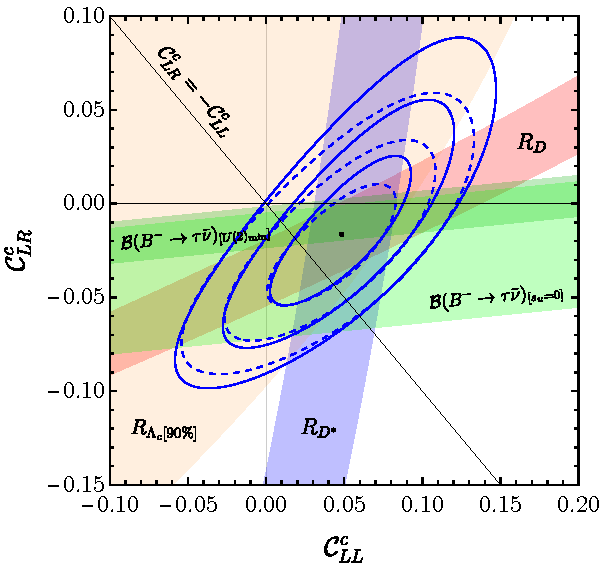
\includegraphics[width=0.74\textwidth]{Figs/CH3/CLL_CLR_lowPT_HFLAV2023.pdf}
    \caption[Fit results in ($C_{LL}^{c}, C_{LR}^{c}$) plane using low-energy observables]{The result in $(C_{LL}^{c},C_{LR}^{c})$ plane obtained from the fit to low-energy $b\rightarrow c\tau\nu$ observables. The blue solid ellipses correspond to the 1, 2 and 3$\sigma$ contours. The blue dotted lines are obtained including also the constraint from $\mathcal{B}(B^{-}_{u}\to \tau\bar{\nu})$. The black point indicates the best-fit point of the fit, $(C_{LL}^{c},C_{LR}^{c})=(0.05,-0.02)$. The coloured bands show the $\Delta\chi^{2}=1$ regions preferred by the individual observables. The pure-left-handed scenario ($\beta_{R}^{33}=0$) and the equal magnitude right-handed scenario ($\beta_{R}^{33}=-1$) are given by the black solid lines~\cite{Aebischer2022}.}
    \label{fig:cll_clr_low_energy_fit}
\end{figure}

\paragraph{Pure-left-handed scenario.}
For $\beta_{R}^{33}=0$, Eq.~\ref{eq:clr_c_approx} gives $C_{LR}^{c}=0$.  Therefore, the $U_{1}$ leptoquark contribution to $b\rightarrow c\tau\nu$ is described only by the left-handed vector operator, as given by Eq.~\ref{eq:cll_c_approx}. This is the primary benchmark scenario considered in this thesis. The corresponding $B$-anomaly-favoured region can be obtained from the intersection of the low-energy fit with the line $C_{LR}^{c}=0$ in Fig.~\ref{fig:cll_clr_low_energy_fit}.

\paragraph{Right-handed scenario.}
The second benchmark is obtained by allowing a sizeable right-handed third-generation coupling. For $\beta_{R}^{33}=-1$, the relation between the Wilson coefficients becomes
\begin{align}
    C_{LR}^{c}=-C_{LL}^{c}.
\end{align}
This benchmark therefore corresponds to the diagonal line in Fig.~\ref{fig:cll_clr_low_energy_fit}, where the right-handed third-generation coupling has the same magnitude as the left-handed coupling.

The two scenarios are described by the parameter space $(\beta_L^{23},\MU,\gU)$ with different fixed values of $\beta_R^{33}$. Particular emphasis is placed on $\beta_L^{23}$, since charged-current low-energy data alone do not provide a stringent constraint on this coupling. For fixed $\MU$ and $\gU$, $\beta_L^{23}$ has a strong impact on $C_{LL}^{c}$ because its contribution is enhanced by the CKM ratio $V_{cs}/V_{cb}$.

Indeed, one can constrain the size of $\beta_L^{23}$ by considering possible ultraviolet (UV) completions of the simplified $U_{1}$ model. While the simplified model parametrises the relevant interactions directly in terms of the couplings $\beta_{L}^{ij}$, the UV completion provides a more fundamental description of their origin. One example is the ``4321'' model, which is based on the extended gauge group $\mathcal{G}_{4321}=SU(4)\times SU(3)'\times SU(2)_L \times U(1)'$. In the flavour structure considered in this model, the $U_1$ couplings are non-universal, with $|\beta_{L}^{23}|<|\beta_{L}^{33}|$~\cite{Cornella2019}.

Additional constraints can be introduced when considering $\Delta F=2$ observables. These are processes in which a quark-flavour quantum number changes by two units, including neutral-meson mixing such as $B_s$--$\bar{B}_s$, $K$--$\bar{K}$, and $D$--$\bar{D}$ mixing. In a given UV completion, the flavour-symmetry breaking that generates non-universal $U_{1}$ couplings may also be transmitted to the neutral-current sector, inducing flavour-changing neutral currents (FCNC) and consequently additional contributions to $\Delta F=2$ processes. The strong experimental constraints on neutral-meson mixing therefore restrict the allowed flavour-violating structure of the UV model and indirectly constrain $\beta_{L}^{23}$.

Combining such considerations of the UV flavour structure with constraints from $\Delta F=2$ observables, Ref.~\cite{Aebischer2022} identifies
\begin{align}
\beta_{L}^{23}\in[0.06,0.16]
\end{align} as a theoretically motivated range for experimental searches. \textbf{However, this constraint should not be interpreted as a model-independent experimental bound on $\beta_{L}^{23}$.} Additional particles, flavour symmetries, or cancellation mechanisms may suppress flavour-changing transitions and thereby allow larger values of $\beta_{L}^{23}$. Therefore, large values of $\beta_{L}^{23}$ remain a possibility within the $U_{1}$ model, and it is important to test this complementary region directly.

% this section is not really important for the discussion, can be added later if necessary.
% \subsection{Ultraviolet completion and the 4321 model}
% \label{subsec:u1_uv_completion}

% The simplified $U_{1}$ model specifies the interactions relevant for
% low-energy and collider phenomenology, but does not determine the
% high-energy origin of the massive vector leptoquark or of its flavour
% structure.
% A UV completion becomes particularly important for loop-induced
% observables that cannot be predicted unambiguously within the
% simplified model alone.
% For example, constraints from $\Delta F=2$ transitions can depend on
% additional heavy particles and flavour-breaking interactions that are
% not specified by the simplified $U_{1}$ Lagrangian~\cite{Cornella2019}.

% A well-motivated class of UV completions is based on the so-called
% 4321 gauge symmetry,
% $$
%     G_{4321}
%     =
%     SU(4)\times SU(3)'\times SU(2)_{L}\times U(1)'.
% $$
% After spontaneous symmetry breaking to the SM gauge group, the broken
% generators of the extended symmetry include a massive vector boson
% with the quantum numbers of the $U_{1}$ leptoquark.
% The $U_{1}$ therefore appears as a gauge boson of an extended
% quark--lepton symmetry rather than as an isolated massive vector field.
% Concrete realisations also contain additional heavy vector bosons and
% vector-like fermions~\cite{Cornella2019,Aebischer2022}.

% Mixing between the SM fermions and the additional vector-like fermions
% can generate a flavour hierarchy in the effective $U_{1}$ couplings.
% In particular, the dominant interaction with third-generation fermions
% can be accompanied by smaller couplings to lighter generations,
% providing a possible dynamical origin for
% $\beta_{L}^{23}\ll\beta_{L}^{33}$.
% The same flavour-breaking structure also contributes to
% flavour-changing neutral-current observables and can therefore impose
% additional constraints on $\beta_{L}^{23}$ within a specific UV model.

% As an illustration, the UV-complete benchmark of
% Ref.~\cite{Cornella2019} gives
% $\beta_{L}^{33}=0.84$ and $\beta_{L}^{23}=0.11$, corresponding to
% \begin{align}
%     \left|
%         \frac{\beta_{L}^{23}}{\beta_{L}^{33}}
%     \right|
%     \simeq 0.13.
% \end{align}
% This benchmark demonstrates that an off-diagonal coupling of order
% $0.1$ can arise naturally in a concrete UV completion.
% It is, however, presented as an illustrative viable point rather than
% as a unique or preferred realisation of the $U_{1}$ model.

% The UV considerations therefore provide a theoretical motivation for
% a hierarchical flavour structure, but they do not define the full
% parameter space of the simplified model.
% The collider search presented in this thesis consequently retains
% $\beta_{L}^{23}$ as a free parameter and tests values beyond those
% typically considered in the 4321 benchmarks.

\subsection{Leptoquark searches at the LHC}
\label{subsec:lq_searches_lhc}

Leptoquarks can be searched for at the LHC through several production modes, including pair production, resonant single production, and non-resonant $t$-channel exchange. Pair production is dominated by QCD interactions. For a fixed $\kappa$ choice, its cross section depends strongly on $\MU$ but weakly on the couplings $\gU$ and $\beta^{i\alpha}$. Pair-production searches therefore provide relatively robust constraints on the leptoquark mass.

ATLAS and CMS have performed searches for pair-produced leptoquarks coupling
to third-generation fermions in final states containing $\tau$-leptons,
$b$-jets, and, depending on the decay mode, missing transverse momentum
~\cite{ATLAS2023LQBTau,CMS2021LQThirdGen}.
For the vector $U_{1}$, the mass limit extends to approximately
$1.5$--$1.8~\TeV$ as shown in Fig.~\ref{fig:lq_atlas_summary_u1}. The limit also depends on the choice of the $U_{1}$--gluon coupling, such as the Yang--Mills or minimal-coupling scenario, as well as on the decay pattern determined by the assumed fermionic couplings.

For single production, the cross section also depends strongly on the leptoquark--fermion couplings. Searches for singly produced leptoquarks decaying into $b\tau$ have been performed in the $b\tau\tau$ final state, where the leptoquark is produced in association with a $\tau$-lepton as shown in Fig.~\ref{fig:lq_single_production}~\cite{ATLAS2023LQBTau,CMS2024LQBTau}. In addition, virtual $t$-channel $U_1$ exchange can contribute to final states such as $\tau\tau$ or $\tau\nu$, enhancing the event yields in the high-mass region. ATLAS and CMS have therefore searched for non-resonant leptoquark contributions in high-mass $\tau\tau$ production ~\cite{ATLAS2025HighMassTauTau,CMS2023TauTauLQ}. These searches can remain sensitive to masses beyond the reach of the direct pair-production searches, particularly for large $\gU$, since the sensitivity is approximately governed by $\gU/\MU$.

\begin{figure}[thbp]
    \centering
    \begin{subfigure}[b]{0.32\textwidth}
        \centering
        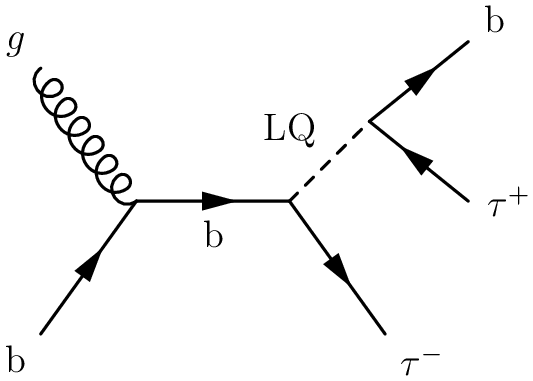
\includegraphics[width=\linewidth]{Figs/CH3/LQ_single_production.png}
        \caption{Single production}
        \label{fig:lq_single_production}
    \end{subfigure}
    \hfill
    \begin{subfigure}[b]{0.32\textwidth}
        \centering
        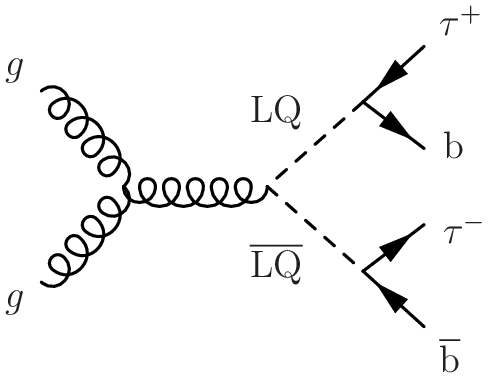
\includegraphics[width=\linewidth]{Figs/CH3/LQ_pair_production.png}
        \caption{Pair production}
        \label{fig:lq_pair_production}
    \end{subfigure}
    \hfill
    \begin{subfigure}[b]{0.32\textwidth}
        \centering
        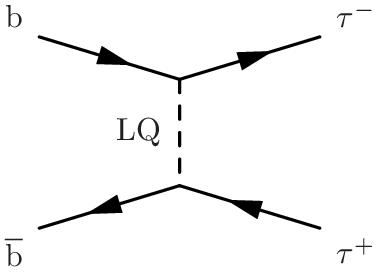
\includegraphics[width=\linewidth]{Figs/CH3/LQ_tchannel_production.png}
        \caption{Non-resonant $t$-channel}
        \label{fig:lq_tchannel_exchange}
    \end{subfigure}

    \caption{Example Feynman diagrams of LQ production and exchange process for $\tau\tau(+b)$ searches.}
    \label{fig:lq_production_modes}
\end{figure}

\begin{figure}[tbp]
    \centering
    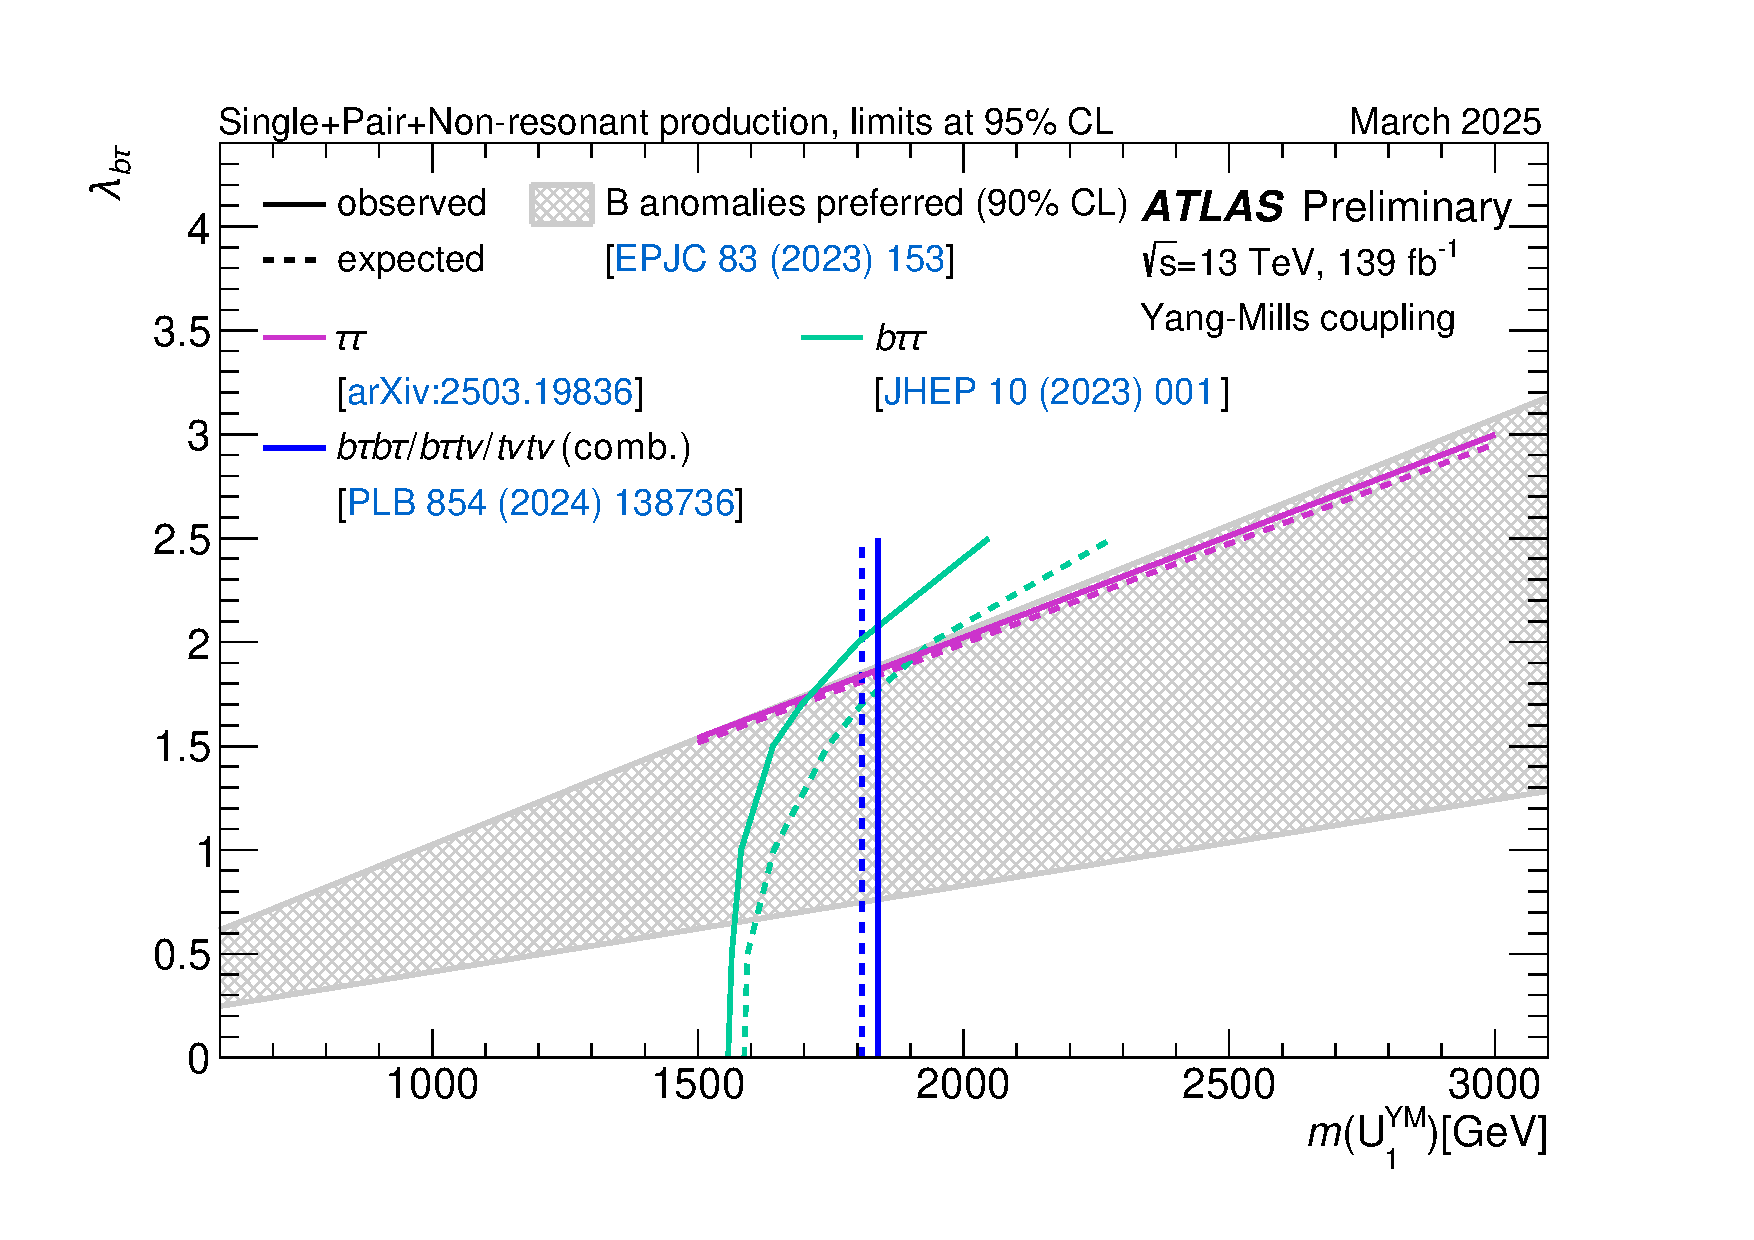
\includegraphics[width=0.72\textwidth]{Figs/CH3/atlas_LQ_summary_u1_ym.pdf}
    \caption[ATLAS constraints on the $U_{1}$ leptoquark]{ Summary of the observed and expected $95\%$ CL constraints on the $U_{1}$ vector-leptoquark coupling $\lambda_{b\tau}$ as a function of the leptoquark mass in the Yang--Mills coupling scenario, with $\beta_R^{33}=0$. Pair-production searches dominate the direct mass constraint at lower masses, while single-production and $\tau\tau$ searches provide coupling-dependent sensitivity at larger masses. Here $\lambda_{b\tau}=\gU/\sqrt{2}$ for $\beta_{L}^{33}=1$~\cite{ATLAS2025LQSummary}.}
    \label{fig:lq_atlas_summary_u1}
\end{figure}

On the other hand, the existing $\tau\tau(+b)$ searches generally assume $\beta_{L}^{23}$ to be small or neglect its contribution, motivated by the flavour assumptions discussed in Sec.~\ref{subsec:u1_low_energy_fit}. Consequently, scenarios with a sizeable $c\nu_{\tau}$ coupling, and in particular the large-$\beta_{L}^{23}$ region, have not been systematically explored at the LHC.

The $\tau\nu$ final state provides a complementary probe of the $b\tau$ and $c\nu_\tau$ coupling. CMS has performed an inclusive search for events with a hadronically decaying $\tau$-lepton and large missing transverse momentum, including an interpretation in terms of leptoquark exchange~\cite{CMS2023TauNu}, but without an explicit $b$-jet requirement. This thesis presents a dedicated search in the $\tau\nu(+b)$ final state. Prior to the analysis, no dedicated ATLAS or CMS leptoquark search had targeted this topology. The $\tau\nu(+b)$ search presented here is therefore complementary to the existing $\tau\tau(+b)$ searches: it probes both the $b\tau$ and $c\nu_{\tau}$ couplings and extends the collider interpretation to large values of $\beta_{L}^{23}$. The corresponding benchmark and target signatures are introduced in the following subsection.

\subsection{Signal model and target signatures}
\label{subsec:lq_collider_benchmark}

In this thesis, we focus on the simplified $U_{1}$ model introduced in Sec.~\ref{subsec:u1_simplified_model} in the Yang--Mills scenario, corresponding to $\kappa_c=\kappa_Y=0$ in Eq.~\ref{eq:u1_full_lagrangian}. The third-generation coupling is normalised to $\beta_{L}^{33}=1$, while the primary interpretation assumes a pure-left-handed scenario ($\beta_{R}^{33}=0$). An additional interpretation including a right-handed coupling is presented with the final results. Therefore, the signal is characterised by $(\MU,\gU,\beta_L^{23})$.

Figure~\ref{fig:u1_taunu_target_topologies} shows representative $U_{1}$ signal diagrams targeted by the analysis. Both resonant single production and non-resonant $t$-channel exchange are considered, and each is divided according to the presence or absence of a $b$-tagged jet. This results in four target signatures: resonant $\tau\nu+b$, non-resonant $\tau\nu+b$, resonant $\tau\nu+0b$, and non-resonant $\tau\nu+0b$.

\begin{figure}[thbp]
    \centering
    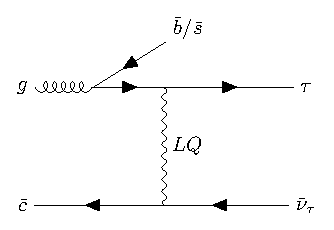
\includegraphics[width=0.43\textwidth]{Figs/CH3/Diagram1.pdf}
    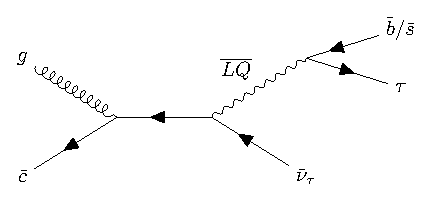
\includegraphics[width=0.43\textwidth]{Figs/CH3/Diagram2.pdf}
    \caption[Signal topologies in the $\tau\nu(+b)$ final state]
    {Signal diagrams targeted in this analysis: non-resonant $t$-channel exchange (left) and resonant single production (right). The final-state jet can originate from a $b$- or $s$-quark.}
    \label{fig:u1_taunu_target_topologies}
\end{figure}

The $b$-jet requirement provides strong discrimination against the dominant SM $\tau\nu+\mathrm{jets}$ background, since genuine SM production of a $\tau\nu$ system in association with a $b$-quark is CKM suppressed ~\cite{Endo2022NonResonant}. The $\tau\nu+b$ categories are therefore particularly sensitive to the combination of the $b\tau$ and $c\nu_{\tau}$ interactions.

The zero-$b$ categories extend the sensitivity to the large $\beta_{L}^{23}$ region explored in this thesis. As $\beta_{L}^{23}$ increases, the $s\tau$ interaction also becomes sizeable, producing signal events without a final-state $b$-quark. This contribution is particularly relevant for resonant production, where an on-shell $U_{1}$ can decay into $s\tau$. The four categories therefore provide complementary sensitivity to the different flavour and production configurations of the $U_{1}$ signal.
